\documentclass[12pt,fleqn,a4paper,oneside]{LegrandOrangeBook}
\addbibresource{sample.bib} % Bibliography file
\definecolor{ocre}{RGB}{103, 61, 76}
\chapterimage{orange1.jpg} 
\chapterspaceabove{6.5cm}
\chapterspacebelow{6.75cm} 
%\begin{theorem}[Name of the theorem]
%\begin{exercise}
%\begin{example}[Example name]
%\begin{definition}[Definition name]
%\begin{corollary}[Corollary name]
%\begin{remark}
%\begin{proposition}[Proposition name]
%\begin{problem}
%\begin{vocabulary}[Word]
%\begin{notation}
%----------------------------------------------------------------------------------------
\begin{document}
%----------------------------------------------------------------------------------------
\section{Introducción}
Como siempre, antes de este curso hay que recordar algunos términos o conceptos para poder entender cosas que se vienen. Empezamos con las unidades logarítmicas:
\begin{align*}
Belio&=\log\left(\frac{P_{out}}{P_{in}}\right)\\
Decibelio(dB)&=10\cdot\log\left(\frac{P_{out}}{P_{in}}\right)\\
Decibelio(dB)&=20\cdot\log\left(\frac{V_{out}}{V_{in}}\right)\\
Neper(Np)&=ln\left(\frac{V_{out}}{V_{in}}\right)
\end{align*}
Asimismo debemos tener en cuenta las demás medidads respecto a un valor como 1mW, 1W, 1V, etc.\footnote{Estas puedes ser vistas en la sección \textbf{Decibelios} en el capítulo de \textbf{Ingeniería en mantenimiento}.}
Otros conceptos importantes a recordar son:
\begin{definition}[Longitud de Onda]
\begin{equation}
\lambda=\frac{v}{f}
\end{equation}
Donde:
\begin{itemize}
\item $\lambda$: Longitud de onda (m)
\item \textbf{v}: Velocidad, si el medio es el aire o espacio libre: v=c=300000 km/s=300000000 m/s (m/s)
\item $f$: Frecuencia (Hz)
\end{itemize}
\end{definition}
\begin{definition}[Temperatura]
\begin{equation}
\frac{°C}{5}=\frac{°F-32}{9}=\frac{K-273}{5}=\frac{R-492}{9}
\end{equation}
Despejando podemos obtener:
\begin{align*}
°C=\frac{5}{9}\left(°F-32\right)\\
K=°C+273\\
R=°F+460
\end{align*}
\end{definition}
Además debemos recordar las bandas y frecuencias designadas por la ITU:
\begin{table}[H]
\centering
\begin{tabular}{|c|c|c|c|}
\hline
\rowcolor[HTML]{9698ED} 
N° de banda & Rango de frecuencia & Indicativo & Propagación                    \\ \hline
2           & 30-300 Hz           & ELF        & Onda terrestre                 \\ \hline
3           & 0.3-3 KHz           & SLF        & Onda terrestre                 \\ \hline
4           & 3-30 KHz            & VLF        & Onda terrestre                 \\ \hline
5           & 30-300 KHz          & LF         & Onda terrestre y superficial   \\ \hline
6           & 0.3-3 MHz           & MF         & Onda superficial               \\ \hline
7           & 3-30 MHz            & HF         & Onda superficial y Ionosférica \\ \hline
8           & 30-300 MHz          & VHF        & Onda Ionosférica y directa     \\ \hline
9           & 0.3-3 GHz           & UHF        & Onda directa                   \\ \hline
10          & 3-30 GHz            & SHF        & Onda directa                   \\ \hline
11          & 30-300 GHz          & EHF        & Onda directa e infrarojo       \\ \hline
12          & 0.3-3 THz           &            & Luz infraroja                  \\ \hline
13          & 3-30 THz            &            & Luz infraroja                  \\ \hline
14          & 30-300 THz          &            & Luz infraroja                  \\ \hline
15          & 0.3-3 PHz           &            & Luz visible                    \\ \hline
16          & 3-30 PHz            &            & Luz ultravioleta               \\ \hline
17          & 30-300 PHz          &            & Rayos X                        \\ \hline
18          & 0.3-3 EHz           &            & Rayos X                        \\ \hline
19          & 3-30 EHz            &            & Rayos cósmicos                 \\ \hline
\end{tabular}
\caption{Designación de bandas CCIR por la ITU.}
\end{table}
Los medios de transmisión:
\begin{table}[H]
\resizebox{\textwidth}{!}{
\begin{tabular}{|c|c|c|c|}
\hline
\rowcolor[HTML]{9698ED} 
Medio de transmisión                                                                         & Banda de frecuencia & Longitud de onda & Aplicación principal                                                                                                                                         \\ \hline
\begin{tabular}[c]{@{}c@{}}Par de alambres,\\ cable multipar\end{tabular}                    & 30-300 Hz           & 10000-1000 Km    & Comunicación submarina                                                                                                                                       \\ \hline
\begin{tabular}[c]{@{}c@{}}Par de alambres,\\ cable multipar\end{tabular}                    & 0.3-3 KHz           & 1000-100 Km      & \begin{tabular}[c]{@{}c@{}}Telefonía, transmisión de datos,\\ telex, fax.\end{tabular}                                                                       \\ \hline
\begin{tabular}[c]{@{}c@{}}Par de alambres,\\ cable multipar,\\ ondas de tierra\end{tabular} & 3-30 KHz            & 100-10 Km        & \begin{tabular}[c]{@{}c@{}}Telefonía de onda portadora baja,\\ capacidad, navegación y radiotelegrafía.\end{tabular}                                         \\ \hline
\begin{tabular}[c]{@{}c@{}}Par de alambres,\\ ondas de tierra\end{tabular}                   & 30-300 KHz          & 10-1 Km          & \begin{tabular}[c]{@{}c@{}}Telefonía de onda portadora mediana\\ capacidad, radiofaro, navegación,\\ radiodifusión onda larga.\end{tabular}                  \\ \hline
\begin{tabular}[c]{@{}c@{}}Cable coaxial, ondas\\ de cielo\end{tabular}                      & 0.3-3 MHz           & 1000-100 m       & \begin{tabular}[c]{@{}c@{}}Radiodifusión, AM, radio aficionados,\\ radio móvil.\end{tabular}                                                                 \\ \hline
\begin{tabular}[c]{@{}c@{}}Cable coaxial, cable UTP cat 3-4,\\ ondas de cielo\end{tabular}   & 3-30 MHz            & 100-10m          & \begin{tabular}[c]{@{}c@{}}Radio aficionados, comunicaciones milirares,\\ marítimas, radio telefonía movil.\end{tabular}                                     \\ \hline
\begin{tabular}[c]{@{}c@{}}Cable coaxial, cable UTP cat 5,\\ ondas directas\end{tabular}     & 30-300 MHz          & 10-1 m           & \begin{tabular}[c]{@{}c@{}}TV, radiodifusión FM, multiacceso radial,\\ radio enlaces, direccionales.\end{tabular}                                            \\ \hline
Ondas directas                                                                               & 0.3-3 GHz           & 100-10 cm        & \begin{tabular}[c]{@{}c@{}}TV, telemetría por radar, comunicaiones\\ militares por satélite, telefonía celular, radio\\ de espectro ensanchado.\end{tabular} \\ \hline
Guía de onda, línea visual                                                                   & 3-30 GHz            & 10-1 cm          & \begin{tabular}[c]{@{}c@{}}Comunicaiones vía satélite, radio enlace\\ direccional analógico y digítal, operación\\ aérea por radar.\end{tabular}             \\ \hline
Guía de onda, línea visual.                                                                  & 30-300 GHz          & 1-0.1 cm         & \begin{tabular}[c]{@{}c@{}}Comunicación militar por satelite, \\ radio astronomia, aterrizaje por radar.\end{tabular}                                        \\ \hline
Fibra óptica                                                                                 & 100-1000 THz        & 3-0.3 pm         & \begin{tabular}[c]{@{}c@{}}Telefonia muy alta capacidad, servicios de\\ banda ancha (SONET, SDH y ATM),\\ video conferencia, CATV por F.O.\end{tabular}      \\ \hline
\end{tabular}
}
\end{table}
\subsection*{Ancho de banda y capacidad de información}
Las limitaciones más importantes para el funcionamiento de una sistema de comunicaciones son el \textbf{ruido} y el \textbf{ancho de banda}. El ancho de banda de un canal de comunicación es la diferencia entre la frecuencia máxima y mínima que puede pasar por el canal. El ancho de banda de un canal de comunicación debe ser igual o mayor que el ancho de banda de la información.
\begin{definition}[Ley de Hartley]
Es la medida de cuanta información se puede transferir a través de un sistema de comunicaciones en un determinado tiempo.
\begin{equation}
I\approx B\times t
\label{eq:hartley}
\end{equation}
Donde:
\begin{itemize}
\item \textbf{I}: Capacidad de información.
\item \textbf{B}: Ancho de banda (Hz)
\item \textbf{t}: Tiempo de transmisión (s)
\end{itemize}
\end{definition}
\begin{notation}
Se requieren \textbf{3 KHz} de ancho de banda para transmitir las señales telefónicas con calidad de voz.\\
Se asignas 200 KHz para transmisión comercial de FM para música, con alta fidelidad.\\
Se requieren casi 6 MHz de ancho de banda para emitir señales de televisión de alta calidad
\end{notation}
Otra medida que debemos saber es:
\begin{definition}[Capacidad de información de un canal digital]
Shannon relacionó la capacidad de información de un canal de comunicaciones, en bits por segundo (bps), con el ancho de banda y la relación señal a ruido: 
\begin{equation}
I=B\cdot\log_2(1+S/N)
\label{eq:shannon}
\end{equation}
Donde:
\begin{itemize}
\item I: Capacidad de información (bps)
\item B: Ancho de banda (Hz)
\item S/N: Relación señal a ruido.
\end{itemize}
\end{definition}
\subsection*{Ruido}
Energía eléctrica no deseable presente en la banda útil del circuito de comunicación. Se puede clasificar el ruido en dos categorías:
\begin{enumerate}
\item \textbf{Correlacionado}: Solo existe cuando hay una señal. Es aquel que se relaciona mutuamente con la señal, y no puede estar en un circuito a menos que haya una señal de entrada.
Se produce por amplificación no lineal, e incluye la distorsión armónica (cuando se producen las armónicas no deseadas de una señal, debido a una amplificación no lineal) y de intermodulación (generación de frecuencias indeseables de suma o diferencia), ya que las dos son formas de distorsión no lineal.

\item \textbf{No Correlacionado}: Está presente siempre, haya o no señal. El ruido No Correlacionado puede sub dividirse en dos categorías generales:
\begin{enumerate}
\item \textbf{El Ruido Externo }es el que se genera fuera del dispositivo o circuito. Hay tres causas principales de ruido Externo:
\begin{enumerate}
\item \textbf{Ruido atmosférico}: Perturbaciones eléctricas naturales. Electricidad estática (rayos)
\item \textbf{Ruido extraterrestre}: Señales eléctricas originadas fuera de la atmósfera terrestre (solar y cósmico)
\item \textbf{Ruido hecho por el hombre}: Su puente principal son mecanismos que producen chispas, ruido industrial (conmutadores, generadores, lámparas fluorescentes)
\end{enumerate}
\item \textbf{El Ruido Interno} es la interferencia eléctrica generada dentro de un dispositivo o circuito. Las causas principales son:
\begin{enumerate}
\item \textbf{Ruido Térmico}: Asociado con el movimiento rápido y aleatorio de electrones libre, producido por la agitación térmica.
\item \textbf{Ruido de Tiempo de Tránsito}: Variación irregular y aleatoria, producida por la modificación de una corriente de portadores, cuando pasa de la entrada a la salida de un dispositivo.
\item \textbf{Ruido de Disparo}: Se debe a la llegada aleatoria de portadoras al elemento de salida de un dispositivo electrónico (diodo, FET, transistor bipolar).
\end{enumerate}
\end{enumerate}
\end{enumerate}
\subsection*{Ruido térmico}
Es el movimiento aleatorio de los electrones libres dentro de un conductor, causado por la agitación térmica.
Llamado también: Movimiento Browniano por su descubridor Robert Brown, Ruido de Johnson en honor a quien lo relacionó con el movimiento de los electrones y Ruido Blanco porque se produce en todas las frecuencias.
\begin{definition}[Potencia de ruido térmico]
\begin{equation}
P_{tn}=K\cdot T\cdot B
\label{eq:ruido termico}
\end{equation}
Donde:
\begin{itemize}
\item $P_{tn}$: Potencia del ruido térmico\footnote{tn:thermal noise o ruido térmico.} (W)
\item \textbf{K:} Constante de Boltzmann= $1.38\times\basedec{-23} J/°K$
\item \textbf{T}: Temperatura absoluta (°K)
\item \textbf{B}: Ancho de banda (Hz)
\end{itemize}
Alternativamente, el ruido térmico puede ser expresado en dBm, para ello debemos usar la siguiente expresión:
\begin{equation}
P_{tn}(dBm)=10\cdot\log\left(\frac{K\cdot T\cdot B}{0.001}\right)
\label{eq:ruido termico log}
\end{equation}
En temperatura ambiente, el ruido térmico ambiente:
\begin{equation}
P_{tn}(dBm)=-174 dBm+10\log(B)
\label{eq:ruido termico ambiente}
\end{equation}
\end{definition}
\begin{definition}[Voltaje ruido térmico]
\begin{equation}
V_{tn}=\sqrt{4\cdot R\cdot K\cdot T\cdot B}
\label{eq:voltaje ruido termico}
\end{equation}
Donde:
\begin{itemize}
\item \textbf{R}: Resistencia interna ($\Omega$)
\item \textbf{$V_{tn}$}: Voltaje RMS del ruido (V)
\end{itemize}
\end{definition}
\begin{notation}
Para la máxima potencia transferencia de potencia $R_L=R_I$.
\end{notation}
\begin{definition}[Relación señal a ruido-SNR]
Es la relación en decibelios entre la potencia de la señal(S) y la potencia del ruido(N):
\begin{equation}
\label{eq:snr}
SNR=10\log_{10}\left(\frac{S}{N}\right)=20\log_{10}\left(\frac{V_s}{V_n}\right)
\end{equation}
\end{definition}
\begin{remark}
El \textbf{factor a ruido} se define como el cociente entre la potencia SNR de entrada y potencia SNR de salida. Por consecuencia, la \textbf{cifra de ruido} es el factor de ruido expresado en dB.
\end{remark}
\begin{notation}
Para voltaje, 6dB indica que la salida es dos veces el valor de la entrada, es decir: Si la entrada es 1, la salida será 2. Para potencia, 3dB indica lo mismo: el valor de la salida es dos veces el valor de la entrada.
\end{notation}
\subsection*{Ángulo crítico}
Debemos recordar ecuaciones como Ley de Snell, dentro de ella una que usaremos es la del \textit{ángulo crítico}:
\begin{center}
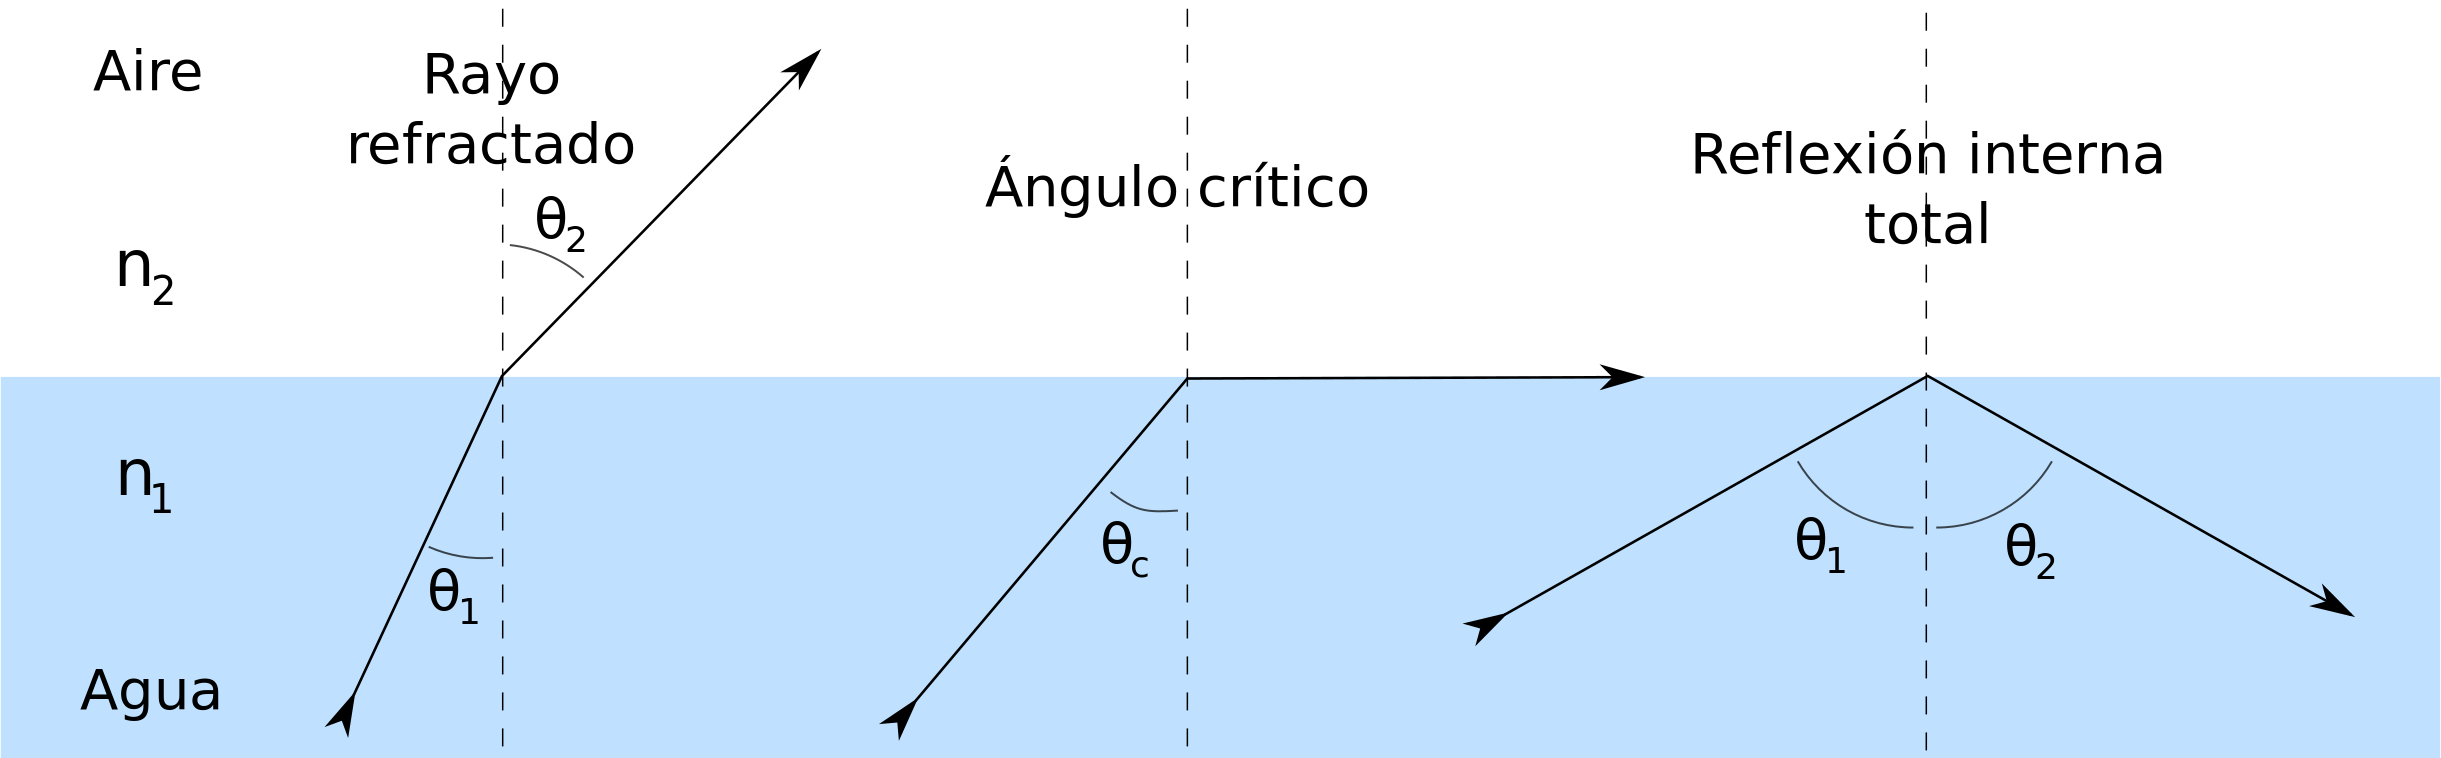
\includegraphics[width=0.8\linewidth]{Ant/Ant1.png}
\end{center}
La forma de obtener el ángulo crítico es:
\begin{equation}
\sin\theta_c=\frac{n_2}{n_1}
\label{eq: angulo critico}
\end{equation}
%----------------------------------------------------------------------------------------
\end{document}
%----------------------------------------------------------------------------------------
